\chapter{État de l'art}

\section{Technologies de communication à distance}


Lors des dernières années, le nombre de dispositifs Internet des Objets (IoT) connaît une croissance fulgurante qui se maintiendra au cours des années qui suivent (voir figure \ref{fig:iot_number}). Ces objets sont capables d’acquérir des données sur leur environnement et/ou de prendre des actions sur celui-ci. Ils communiquent avec d’autres machines pour transmettre les informations acquises et recevoir des commandes lorsque cela est nécessaire. Les dispositifs IoT ont de diverses applications telles que les thermostats intelligents, les voitures connectées, suivi et monitorage d’actifs, et bien d’autres. Selon les conditions d’utilisation et son objectif, ces dispositifs doivent être capables d’envoyer des données sur des courtes ou des longues distances. En outre, leur consommation énergétique doit généralement rester faible, notamment lorsqu’ils sont alimentés par une batterie.

~

\begin{figure}[ht!]
  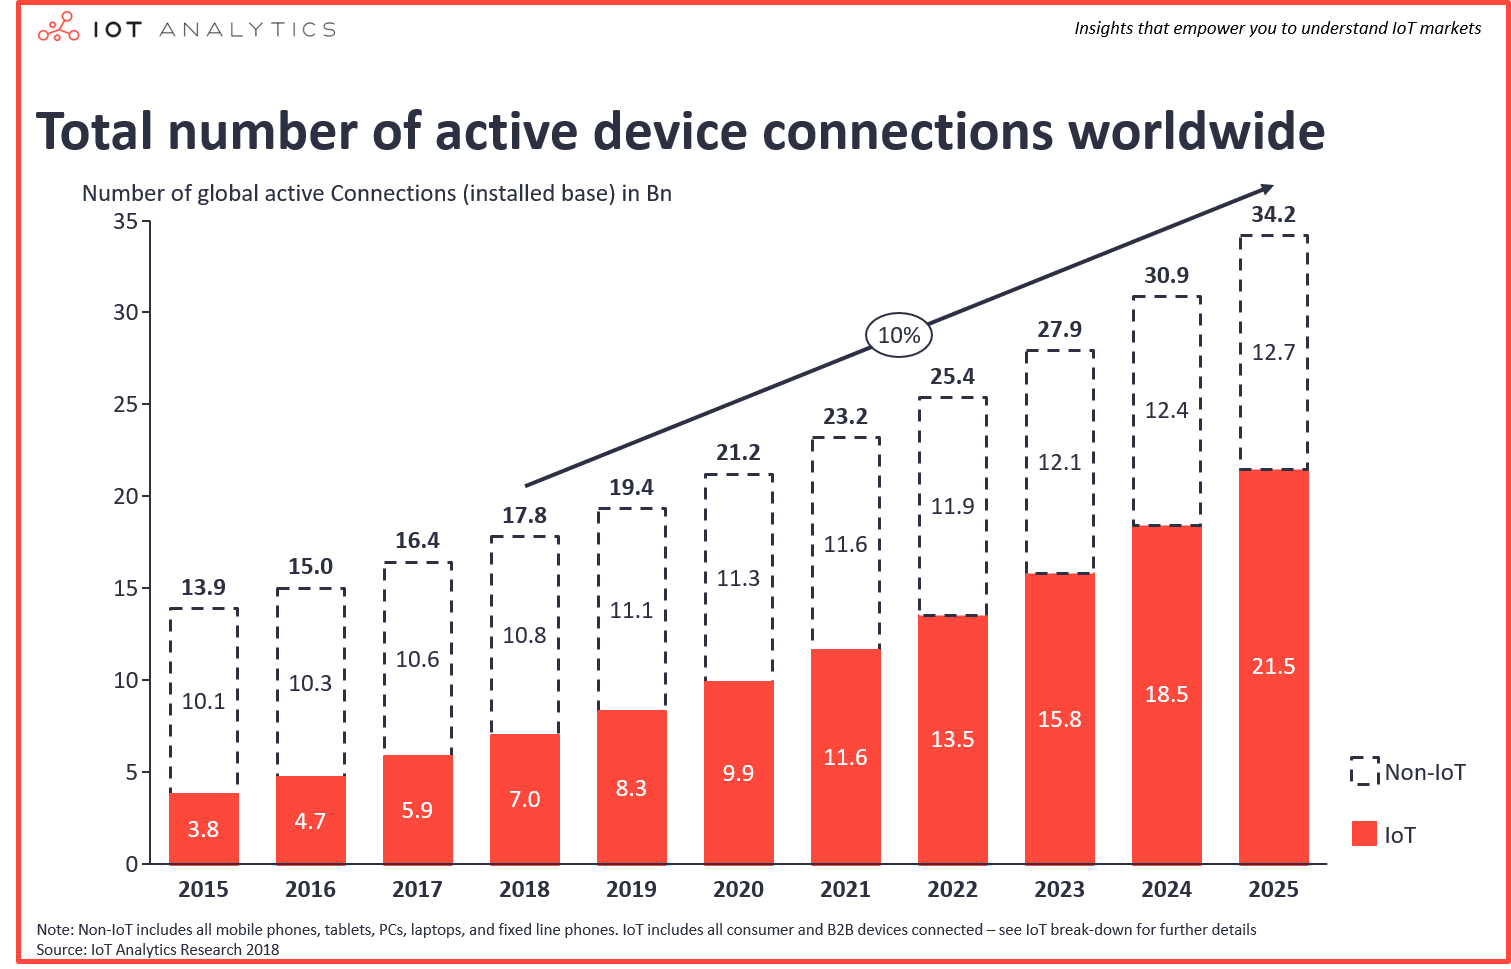
\includegraphics[width=\textwidth]{img/state_of_the_art/iot_number_connected.png}
  \caption{Nombre de dispositifs connectés à Internet \cite{lueth_2018}}
  \label{fig:iot_number}
\end{figure}

~

\noindent
Un réseau de communication unique et employable indépendamment du contexte du projet n’existe pas \cite{vannieuwenborg_iot}. Toutefois, une multitude de réseaux avec des caractéristiques distinctes sont disponibles, tels que LoRaWAN et GSM. La figure 1 présente l’architecture simplifiée des réseaux utilisés par les dispositifs IoT pour échanger des informations avec des serveurs ou des utilisateurs qui sont connectés à Internet. Nous ne nous intéressons ici qu’aux technologies responsables de la transmission de données dans la phase 1 de la figure.

~

\begin{figure}[ht!]
  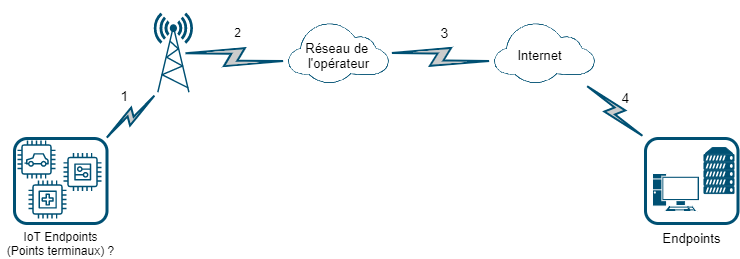
\includegraphics[width=\textwidth]{img/state_of_the_art/network_iot.png}
  \caption{Architecture simplifiée d'un réseau avec dispositifs IoT (Basé sur \cite{sanchez2016state, mekki2018overview})}
  \label{fig:network_archi}
\end{figure}

~

\noindent
Actuellement, les principaux réseaux sans fil disponibles pour les dispositifs IoT sont :

\begin{itemize}
  \item LoRaWAN
  \item Réseaux mobiles (2G/3G/4G/5G)
  \item Sigfox
  \item Satellite
  \item Wi-Fi
  \item Zigbee
  \item Bluetooth
  \item Réseaux mobiles IoT (NB-IoT et LTE-M)
\end{itemize}

~

\noindent
Ces technologies utilisent toutes des ondes électromagnétiques pour transmettre les données, mais les fréquences sur lesquelles elles opèrent sont parfois très différentes. Certaines technologies utilisent une implémentation propriétaire, d’autres se basent sur des standards open source. \cite{foubert_iot} De façon similaire, certaines technologies exploitent la bande ISM\footnote{Bande industrielle, scientifique et médicale}, alors que d’autres exploitent des fréquences non réglementées. Ces dernières permettent de déployer son propre réseau privé, à condition d’acheter et configurer tout le matériel requis ce qui peut demander un investissement initial assez important. Ces différences accordent des propriétés distinctes aux réseaux en ce qui concerne le coût d’utilisation et déploiement, la bande passante, et la portée du signal. À noter également, certains réseaux imposent une taille maximale sur chaque message, qu’il soit envoyé ou reçu. Le tableau comparatif de l’annexe \ref{ap:table_network} offre une vue d’ensemble sur les différentes technologies et leurs propriétés. Il faut cependant remarquer que la portée et le débit sont juste donnés à titre comparatif et ils sont à prendre avec des pincettes. En effet, ces valeurs varient beaucoup en fonction de certains paramètres tels que la géographie du milieu (urbain ou rural) et des éventuelles interférences. Néanmoins, le débit et la portée sont très importants pour classifier ces réseaux et, avec l’aide de la figure \ref{fig:range_iot}, ces technologies peuvent être classées de la façon suivante \cite{orange_iot} :


\begin{figure}
  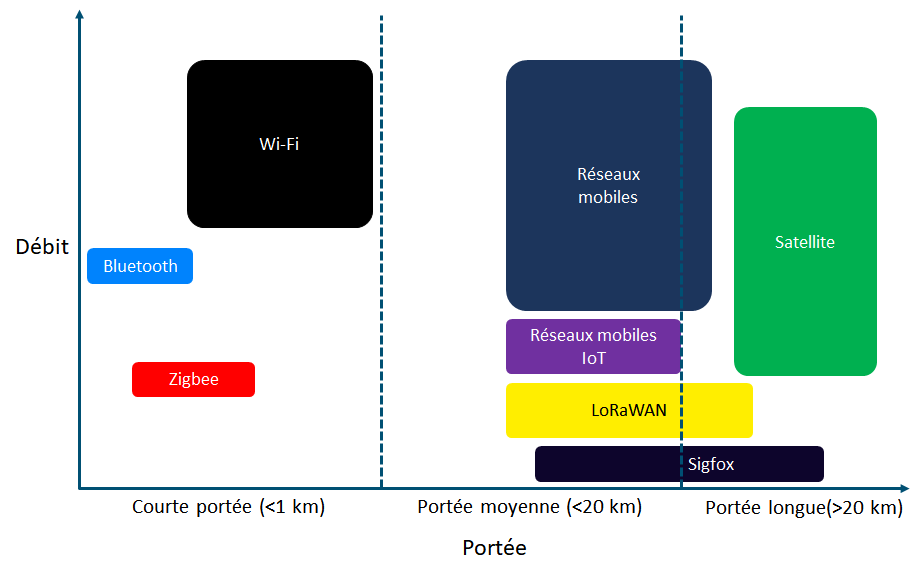
\includegraphics[width=\textwidth]{img/state_of_the_art/range_iot.png}
  \caption{Classement des réseaux en fonction de leur portée et débit (Basé sur )}
  \label{fig:range_iot}
\end{figure}

\begin{itemize}
  \item IoT haut débit : Dans cette catégorie se trouvent principalement les technologies comme les réseaux mobiles, le Wi-Fi et le satellite. Les débits proposés sont généralement supérieurs au Mb/s. En contrepartie, l'utilisation de ces technologies engendre une consommation énergétique plus élevée.
  \item IoT bas débit : Ici se trouvent les réseaux mobiles IoT, LoRaWAN, Sigfox, et Zigbee. En fonction du réseau, le débit peut varier entre quelques bits par seconde jusqu'à un Mb/s. Ces technologies offrent une consommation énergétique faible.
  \item IoT critique : C'est-à-dire lorsqu'il s'avère nécessaire de transmettre des données sur un intervalle de temps donné \cite{orange_iot}. C'est une propriété des réseaux 5G.
\end{itemize}

~

\noindent
Un point également important est que ces technologies ont de différents niveaux de maturité. Au moins un réseau mobile est disponible dans chaque pays, mais les nouveaux réseaux comme Sigfox, LoRaWAN, et 5G sont en revanche toujours en cours de déploiement. De ce fait, ces dernières technologies ne sont disponibles que dans certaines régions possédant une infrastructure moderne. La couverture du réseau est un critère très important à considérer avant effectuer tout choix afin d’éviter de mauvaises surprises.
Finalement, toujours dues à ce différent degré de maturité, certaines technologies plus anciennes pourraient voir la fin de ses jours dans les années à venir. Par exemple, certains opérateurs vont décommissionner leur réseau 2G à partir de 2020 \cite{swisscom_2g}. Les opérateurs restants devraient suivre la même tendance dans les années suivantes. De plus, le réseau 3G devrait suivre la même tendance comme affichée sur la figure \ref{fig:evo_network}.

\begin{figure}[ht]
  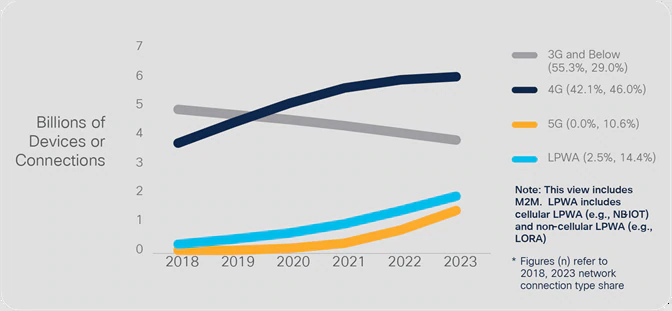
\includegraphics[width=\textwidth]{img/state_of_the_art/network_evolution.png}
  \caption{Évolution du nombre de dispositifs connectés aux différents réseaux \cite{report_cisco}}
  \label{fig:evo_network}
\end{figure}



\section{Monitoring de l'état d'un serveur linux}

La nécessité de surveiller toute l’infrastructure IT, et en particulier des serveurs tournant sous Linux, existe depuis un bon nombre d’années. Cependant, surveiller un système n’est pas trivial. Cela peut être accompli de différentes manières en fonction des évènements ou statistiques qui doivent être observées dans la machine hôte. Par exemple, l’utilisation de logs pour débugger une application ou voir l’historique de transactions d’une base de données est une technique de monitoring utilisée depuis de nombreuses années. D’autres techniques de monitoring existantes sont le profiling, le tracing et l’acquisition de métriques \cite{brazil2018prometheus}. Dans cette section, seulement les technologies d’acquisition de métriques sont présentées puisqu’elles sont les plus utiles pour connaître l’état de la machine.

~

\noindent
Créé à la fin des années 80, le protocole SNMP \cite{RFC1098, RFC1157} permet de monitorer et configurer de différents dispositifs connectés au réseau. Au long des années, des solutions de monitorage de métriques de plus haut niveau, ou tout-en-un, sont apparues sur le marché. Ces solutions utilisent différents protocoles, dont SNMP, pour surveiller les dispositifs sur le réseau et stockent toutes les informations recueillies sur une base de données. De plus, elles permettent de définir un ensemble de conditions à surveiller de plus près et si une de ces conditions est violée, une alerte est transmise vers l’équipe responsable de l’infrastructure. Deux exemples de solutions créées à la fin des années 90 et qui demeurent disponibles sont Nagios et Zabbix.

~

\noindent
Actuellement, un grand nombre de solutions de monitoring sont disponibles sur le marché proposant différents modèles commerciaux. En effet, certaines solutions sont vendues comme un produit, mais d’autres préfèrent suivre un modèle open source. Dans le cas de ces dernières, les entreprises responsables de l’application proposent souvent leurs services en matière d’assistance technique afin d'installer et maintenir la solution. Un autre modèle aussi appliqué est de proposer une version gratuite avec un nombre limité de fonctionnalités, et une version payante débloquant toutes les capacités de l’application. Avant d’entamer toute recherche d’une solution, il faut comprendre quelle formule s’adapte le mieux aux besoins de l’utilisateur.
Comme il est affiché sur la figure \ref{fig:mon_archi}, deux architectures existent pour les solutions de monitoring : \textit{pull} et \textit{push} \cite{brazil2018prometheus, techhub_monitoring, blog_monitoring, techhub_monitoring}. Chaque application est entièrement basée sur une de ces deux approches. Dans certains cas, une solution peut parfois supporter les deux architectures (voir exemple figure \ref{fig:archi_prom_simple}). Cependant, ces solutions détiennent toujours un modèle préféré, et l’autre possibilité sert juste à combler certaines lacunes du premier modèle puisque, en effet, chaque architecture possède ses avantages et faiblesses.

~

\begin{figure}[ht!]
  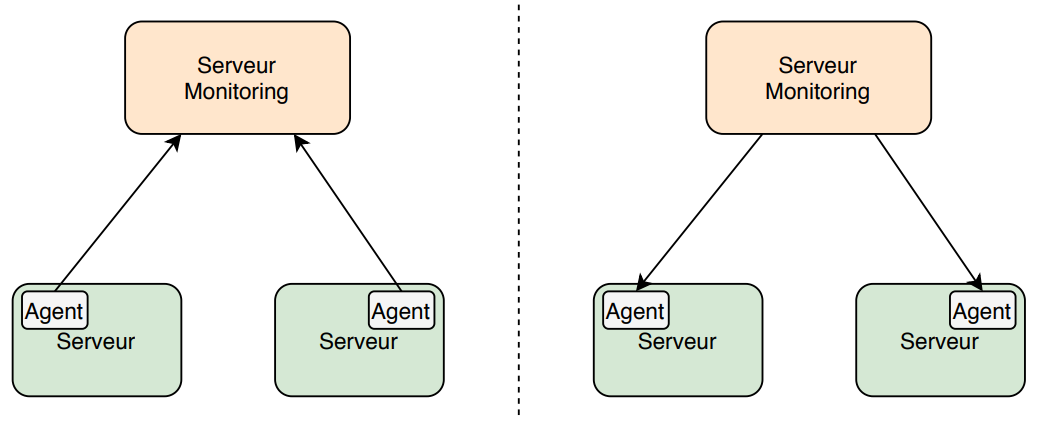
\includegraphics[width=\textwidth]{img/state_of_the_art/monitoring_architecture.png}
  \caption{\textbf{Gauche :} Solution de monitoring avec architecture \textit{push}.  \textbf{Droite :} Solution de monitoring avec architecture \textit{pull}.}
  \label{fig:mon_archi}
\end{figure}



\begin{figure}[ht!]
  \centering
  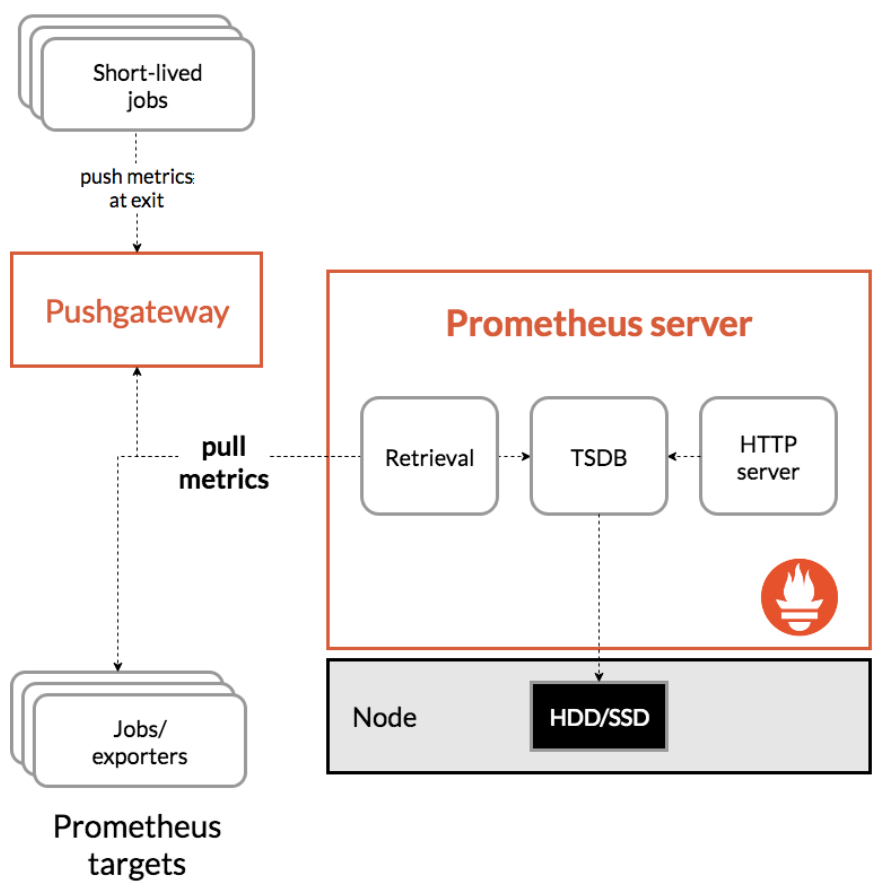
\includegraphics[scale=0.4]{img/state_of_the_art/prometheus_archi_simple.png}
  \caption{Architecture \textit{pull} de Prometheus. Le modèle \textit{push} est supporté grâce au Pushgateway.}
  \label{fig:archi_prom_simple}
\end{figure}

~

\noindent
Dans le modèle de type \textit{push}, les agents dans la machine hôte envoient un ensemble de métriques ou des événements au serveur de monitoring. Cette technique permet notamment de définir des conditions d’alerte dans l’agent, et c’est celui-ci qui se charge de vérifier ces conditions. Lorsque le test des conditions passe, l’agent transmet un événement au serveur de monitoring. De plus, seul le système de push est capable de correctement acquérir des données à propos de jobs Batch de courte durée. \cite{blog_monitoring, prometheus_tuto} En effet, comme affiché sur la figure \ref{fig:batch_end}, le modèle \textit{pull} peut rater la fin du job ce qui se traduit par une perte d’informations.

~

\begin{figure}[ht!]
  \centering
  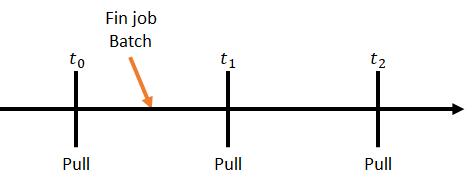
\includegraphics{img/state_of_the_art/pull_batch_miss.png}
  \caption{Faiblesse du modèle \textit{pull}. Le système de monitoring a raté les informations de la fin du job}
  \label{fig:batch_end}
\end{figure}

~

\noindent
Dans le modèle de type \textit{pull}, les agents dans la machine hôte collectent et exposent les métriques, mais c’est au serveur de monitoring d’activement aller retrouver ces données. Par conséquent, les événements et alertes au niveau des agents ne sont pas pris en charge, dans la mesure où ces derniers ne savent pas quand le système de monitoring récupérera les informations. En revanche, cette méthode permet de mieux identifier si un problème s'est produit sur la machine hôte puisqu’elle ne répondra plus aux requêtes lorsque cela a lieu.\cite{prometheus_doc_pull_push} Ceci rend l’approche \textit{pull} légèrement plus fiable que la technique \textit{push}. Les deux méthodes possèdent donc leurs avantages et inconvénients qu’il faut tenir en compte lors du choix de la technologie. Cependant, dans la majorité des cas, les deux architectures offrent ces capacités très similaires \cite{interview_push_pull}.

~

\noindent
Indépendamment de l’architecture utilisée, toutes les informations recueillies ou reçues par le serveur de monitoring doivent être stockées sur une base de données. Les solutions plus anciennes comme Nagios et Zabbix, utilisent principalement des bases de données relationnelles \cite{nagios_db, zabbix_db}. Ceci n’est plus le cas pour les solutions plus récentes telles que Prometheus et le TIG Stack\footnote{Le TIG stack est la combinaison de Telegraf, InfluxDB et Grafana pour créer un outil de monitoring} qui utilisent des bases de données orientées séries temporelles pour la persistance des données. Cette sorte de base de données, comme son nom indique, est mieux optimisée pour des valeurs horodatées \cite{time_series_fr}. En effet, ces bases de données possèdent les propriétés suivantes \cite{alibaba_timeseries}:

\begin{itemize}
  \item Elles supportent des écritures simultanées et avec de grands débits. Typiquement, dans ces bases de données se produisent énormément d’écritures, mais pas beaucoup d’accès.
  \item Ces bases de données doivent stocker d’énormes quantités de données temporelles. Elles utilisent des algorithmes de compression spécifiques pour stocker les données de manière efficace. \cite{di2007efficient}
  \item Toutes les requêtes sont effectuées sur base d’un intervalle dans le temps
  \item Les données ont une durée de rétention. À partir d’une certaine date, la base de données élimine automatiquement les informations car elles sont jugées non utiles.
\end{itemize}

~

\noindent
De ce fait, les bases de données orientées séries temporelles offrent un stockage plus efficace pour les métriques surveillées. Un dernier aspect très important d’une solution de monitoring est la visualisation de données. La majorité des solutions offrent soit un outil de visualisation propriétaire (Nagios ou Zabbix), soit elles exploitent des outils existants tels que Grafana (Prometheus et le TIG Stack).




\section{Plateformes de visualisation de données}
